\documentclass{revtex4-1}

\usepackage{amsmath}

\usepackage{bm}

\usepackage{physics}

\usepackage{graphicx}
\usepackage{subcaption}
\usepackage{epstopdf}
\graphicspath{{img/}}

\everymath{\displaystyle}

\begin{document}

\title{Restricted Boltzmann Machines}
\author{Giancarlo Fissore}
\date{May 2017}

\begin{abstract}
  Abstract text
\end{abstract}

\maketitle

\section{Introduction}

\section{Overview of Restricted Boltzmann Machines}
A Restricted Boltzmann Machine (RBM) is a model for neural networks which basically consists in a bipartite graph with a layer of hidden units \(h_i\) and a layer of visible units \(v_i\). The units in one layer are not connected among them but are connected to all the units in the other layer, as shown in fig. \ref{fig:rbm}. We restrict our treatment to the case of binary units \(h_i,v_i = 0,1\). Drawing a comparison between RBMs and spin models in statistical physics, we can define the following \textit{energy function}

\begin{equation}
E(\textbf{h},\textbf{v}) = - \sum_i a_i v_i - \sum_j b_j h_j - \sum_{i,j} v_i w_{ij} h_j
\end{equation}

where \(a_i\) and \(b_i\) are \textit{external fields} acting respectively on the visible and hidden units. The probability of a certain configuration is then given by the Boltzmann measure (taking \(\beta = 1\))

\begin{equation}
P(\textbf{h},\textbf{v}) = \frac{e^{-E(\textbf{h},\textbf{v})}}{Z}
\end{equation}

where \(Z = \sum_{\textbf{h},\textbf{v}} e^{-E(\textbf{h},\textbf{v})}\) is the \textit{partition function}. The probabilities of activations for visible and hidden units can be simply computed to be

\begin{align}
P(v_i = 1 | \textbf{h}) &  = \frac{1}{1+e^{-a_i - \sum_{j} w_{ij} h_j}} \nonumber \\
& = \sigma \left(a_i + \sum_{j} w_{ij} h_j \right) \\
P(h_j = 1 | \textbf{v}) & = \frac{1}{1+e^{b_j + \sum_i w_{ij} v_i}} \nonumber \\
& = \sigma \left(b_j + \sum_i w_{ij} v_i \right)
\end{align}

\begin{figure}
  \centering
  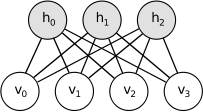
\includegraphics{rbm.png}
  \caption{bipartite structure of a RBM}
  \label{fig:rbm}
\end{figure}

We see that the usual neuron activation function (the sigmoid function, which we indicated by \(\sigma\)) comes out naturally by choosing binary units. Moreover, we can now understand the importance of the external fields: they drive the activation of a certain unit by setting a threshold that has to be overcome by the opposite layer through the couplings \(w_{ij}\).

What we are interested in is the probability for the visible units, which is the layer we use to represent data. It can be easily defined as

\begin{align}
P(\textbf{v}) &  = \sum_{\textbf{h}} P(\textbf{h},\textbf{v}) \nonumber \\
& = \frac{e^{-F(\textbf{v})}}{Z}, \quad Z = \sum_{\textbf{v}} e^{-F(\textbf{v})}
\end{align}

where, further exploiting the parallel with spin models, we have introduced the \textit{free energy}

\begin{align}
F(\textbf{v}) & = -\log \sum_{\textbf{h}} e^{-E(\textbf{h},\textbf{v})} \nonumber \\
& = -\sum_i a_i v_i -\sum_j \log \sum_{h_j} e^{h_j \left( b_j + \sum_i w_{ij} v_i \right)} \nonumber \\
& = -\sum_i a_i v_i -\sum_j \log \left( 1 +  e^{\left( b_j + \sum_i w_{ij} v_i \right)} \right)
\end{align}

To use the RBM as a generative model, we want to maximize \(P(\textbf{v}\)) (and thus minimize the free energy) for the samples belonging to the training set. Once this is done, we can sample the equilibrium configurations of the RBM to obtain samples which are generated according to the probability distribution of the training data. The algorithms used to train and sample RBMs are usually based on Monte Carlo methods. In particular, the most effective algorithms for training are \textit{k-steps contrastive divergence} (CDk) \cite{Hinton_CD}  and \textit{persistent contrastive divergence} (PCD) \cite{PCD}. 

[include a section on TAP]

\section{Singular Values Decomposition of a RBM}
The structure of the samples that a RBM  is able to generate must be in some way encoded into the external fields \(\textbf{a},\textbf{b}\) and the weights matrix \(\textbf{W}\), as these are the set of quantities which constitute the RBM itself. For what concerns the visible field values \(a_i\), these are used to make sure that the visible unit \(i\) is activated with a probability \(p_i\) given by the proportion of training samples in which unit \(i\) is active (i.e. where its value is 1). No learning is needed to make the field \(\textbf{a}\) encode this information, it is sufficient to use the initialization rule

\begin{equation}
a_i = \log[p_i/(1-p_i)]
\label{eq:bias_init}
\end{equation}

as reported in \cite{Hinton_guide}. To understand how the structure of the data is encoded into the weights matrix, instead, we monitored the singular value decomposition (SVD) of \textbf{W} during the training.

\subsection{Informal introduction to Singular Value Decomposition (SVD) and Principal Component Analysis (PCA)}
The Principal Component Analysis (PCA) technique can be introduced by considering the covariance matrix of a dataset. Given a \(n \times p\) data matrix \textbf{\(X\)} where the samples are arranged by rows and centered (i.e. column means have been subtracted), we can define the related covariance matrice (square and symmetric)

\begin{equation}
\textbf{C} = \frac{\textbf{X}^T \textbf{X}}{n-1}
\end{equation}

that can be diagonalized

\begin{equation}
\textbf{C} = \textbf{V L V}^T
\end{equation}

where the columns of \textbf{\(V\)} are eigenvectors of \textbf{\(C\)} and \textbf{\(L\)} is the diagonal matrix of the eigenvalues \(\lambda_i\). Projecting the samples over the eigenvectors of the covariance matrix (also called \textit{principal directions} in the context of PCA) we obtain the \textit{principal components}: new, independent variables that account for the maximum possible variability in the data. More precisely, the first \textit{principal component} maximizes the variance of the projections of the data (i.e. it has the highest possible variance) and the succeeding components maximize the variance while satisfying the constraints of being orthogonal to the preceeding components. A rigorous demonstration of the properties of \textit{principal components} is given in [].

The Singular Value Decomposition (SVD) is the generalization of eigenmodes decomposition to rectangular matrices, and it is given by

\begin{equation}
\textbf{X} = \textbf{U \(\Sigma\)} \textbf{V}^T
\end{equation}

where \(\textbf{U}\) is an orthogonal \(n \times p\)  matrix whose columns are the \textit{left singular vectors} \(\mathbf{\mu}_j \), \textbf{\(V\)} is an orthogonal \(p \times p\) matrix whose columns are the \textit{right singular vectors} \( \mathbf{\nu}_j \) and \( \textbf{\(\Sigma\)} \) is a diagonal \(p \times p\) matrix whose elements are the singular values \(\sigma_j\). The separation into left and right singular vectors is due to the rectangular nature of the decomposed matrix, and the similarity with eigenmodes decomposition is revealed by the following SVD equations

\begin{align}
\mathbf{X \nu} & = \textbf{\(\sigma \mu\)} \\ \nonumber
X^T \mu & = \sigma \nu
\end{align}

Plugging the SVD of \textbf{\(X\)} into the definition of covariance matrix

\begin{align}
C & = \frac{X^T X}{n-1} = \frac{V \Sigma U^T U \Sigma V^T}{n-1}  \\ \nonumber
& = V \frac{\Sigma^2}{n-1} V^T \nonumber 
\end{align}

we see how the \textit{right singular vectors} can be identified as the \textit{principal directions} and a relation between the singular values \(\sigma_j\) and the eigenvalues of the covariance matrice \(\lambda_j\) is easily found

\begin{equation}
\lambda_j = \frac{\sigma_j}{n-1}
\label{eq:ls_map}
\end{equation}

Finally, the \textit{principal components} are given by \(U \Sigma\) (\(XV = U \Sigma V^T V = U \Sigma\)).

[mean-field equations]

In the context of a RBM, we can better specify the role of the SVD matrices:

\begin{itemize}
\item \textbf{U} encodes the singular vectors related to the visible layer and can therefore be visualized in the pixel space
\item  \textbf{V} is related to the hidden layer and it is a square orthogonal matrix that can be interpreted as a rotation. 
\item The singular values \( {\sigma}_j \) contained in \textbf{\(\Sigma\)} can be thought of as scaling factors whose action is to weight the singular vectors composing \textbf{W}.
\end{itemize}

Given the above characteristics we focused our attention on \textbf{\(\Sigma\)} and \textbf{U}, tracking the distribution of the singular values and looking at the corresponding left singular vectors during the training.

\subsection{Distribution of the singular values}
The weights matrix W is initialized as a gaussian random matrix with variance \(\sigma_v\) (and zero mean). The eigenvalues distribution of the corresponding symmetric square matrix \(\mathbf{W}^T \mathbf{W} \) is known to be given by the Marchenko-Pastur law \cite{MP_law} in its canonical form. The singular values \(\sigma_j\) are related to the eigenvalues \(\lambda_j\) by \eqref{eq:ls_map}, and by defining the parameter \( r = p/d \), with \(p\) the size of the hidden layer and \(d\) the size of the visible layer (we recall that \(\mathbf{W}\) is a \(d \times p\) matrix), the expression of the Marchenko-Pastur law is given by (in the limit \( p,d \to \infty \) with \(r\) finite)

\begin{equation}
\rho (\lambda) = \frac{1}{2 \pi \sigma_v^2} \frac{\sqrt{(\lambda - r_-)(r_+ - \lambda)}}{r \lambda}
\end{equation}

where the higher and lower bounds \(r_{\pm}\) are

\begin{equation}
r_{\pm} = \sigma_v^2 \left(1 \pm \sqrt{r} \right)^2
\end{equation}

Fig. \ref{fig:mp_fit} shows the agreement between the empirical distribution and the theoretical distribution. In particular, we note how all \(\sigma_j\) have values below the threshold set by the Marchenko-Pastur law, forming a \textit{bulk} of singular values.

\begin{figure}
  \centering
  \begin{subfigure}{.45\linewidth}
    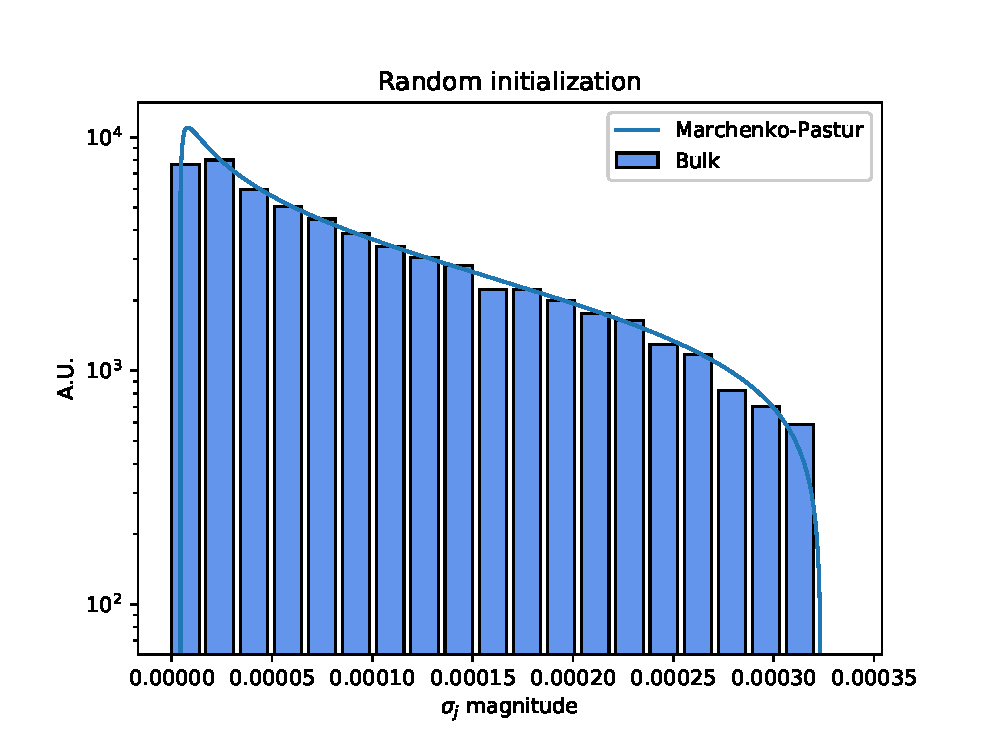
\includegraphics[width=\linewidth]{mp_fit.eps}
    \caption{}
    \label{fig:mp_fit}
  \end{subfigure}
  \begin{subfigure}{.45\linewidth}
    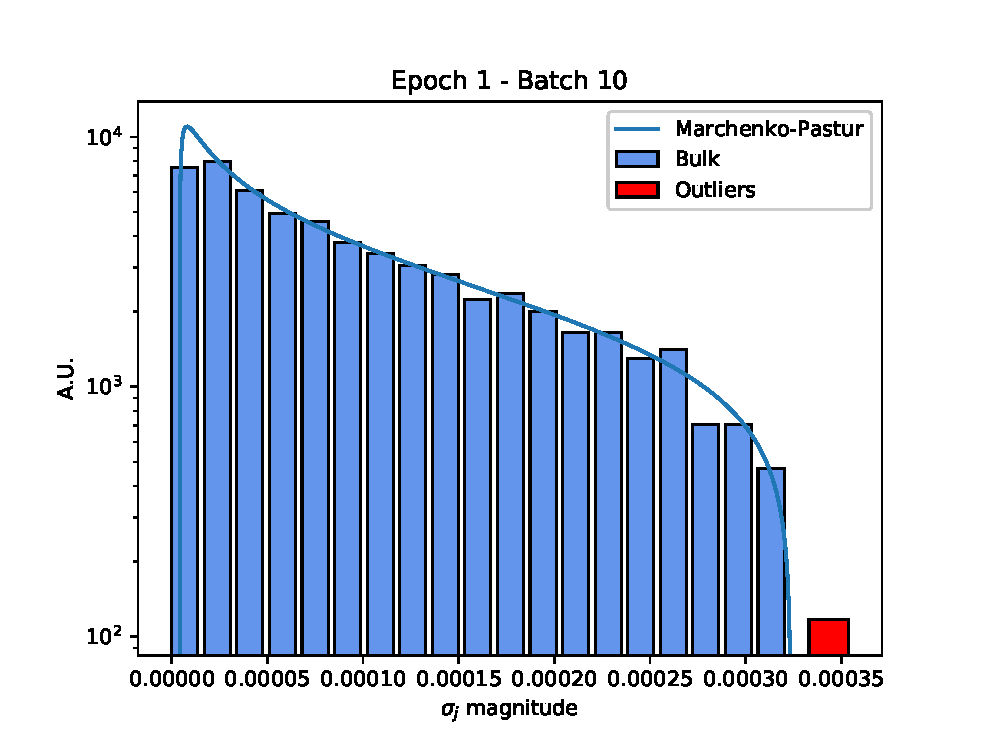
\includegraphics[width=\linewidth]{sv_distr_e1_b10.eps}
    \caption{}
    \label{fig:sv1}
  \end{subfigure}\par\medskip
  \begin{subfigure}{.45\linewidth}
    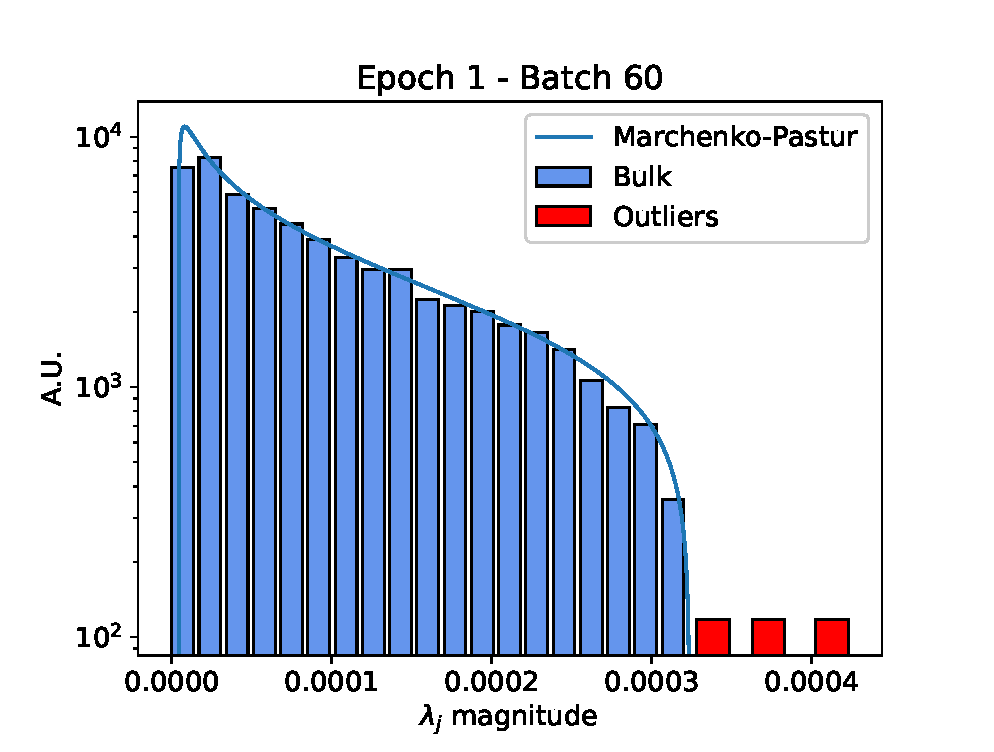
\includegraphics[width=\linewidth]{sv_distr_e1_b60.eps}
    \caption{}
    \label{fig:sv2}
  \end{subfigure}
  \begin{subfigure}{.45\linewidth}
    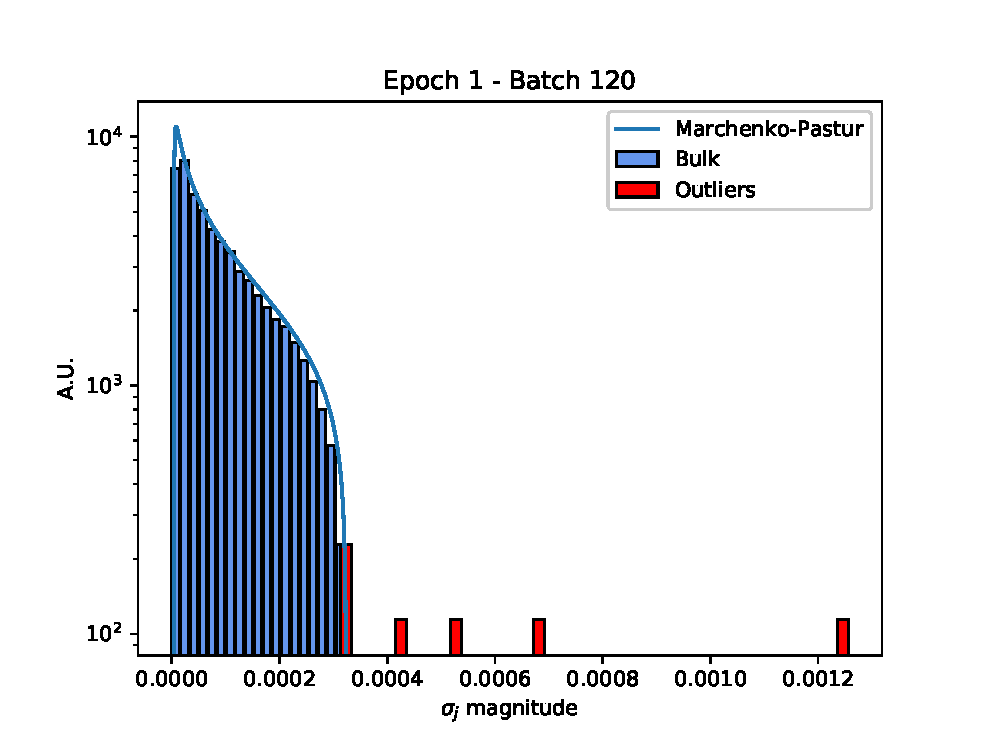
\includegraphics[width=\linewidth]{sv_distr_e1_b120.eps}
    \caption{} 
    \label{fig:sv3}
  \end{subfigure}
  \begin{subfigure}{.5\linewidth}
    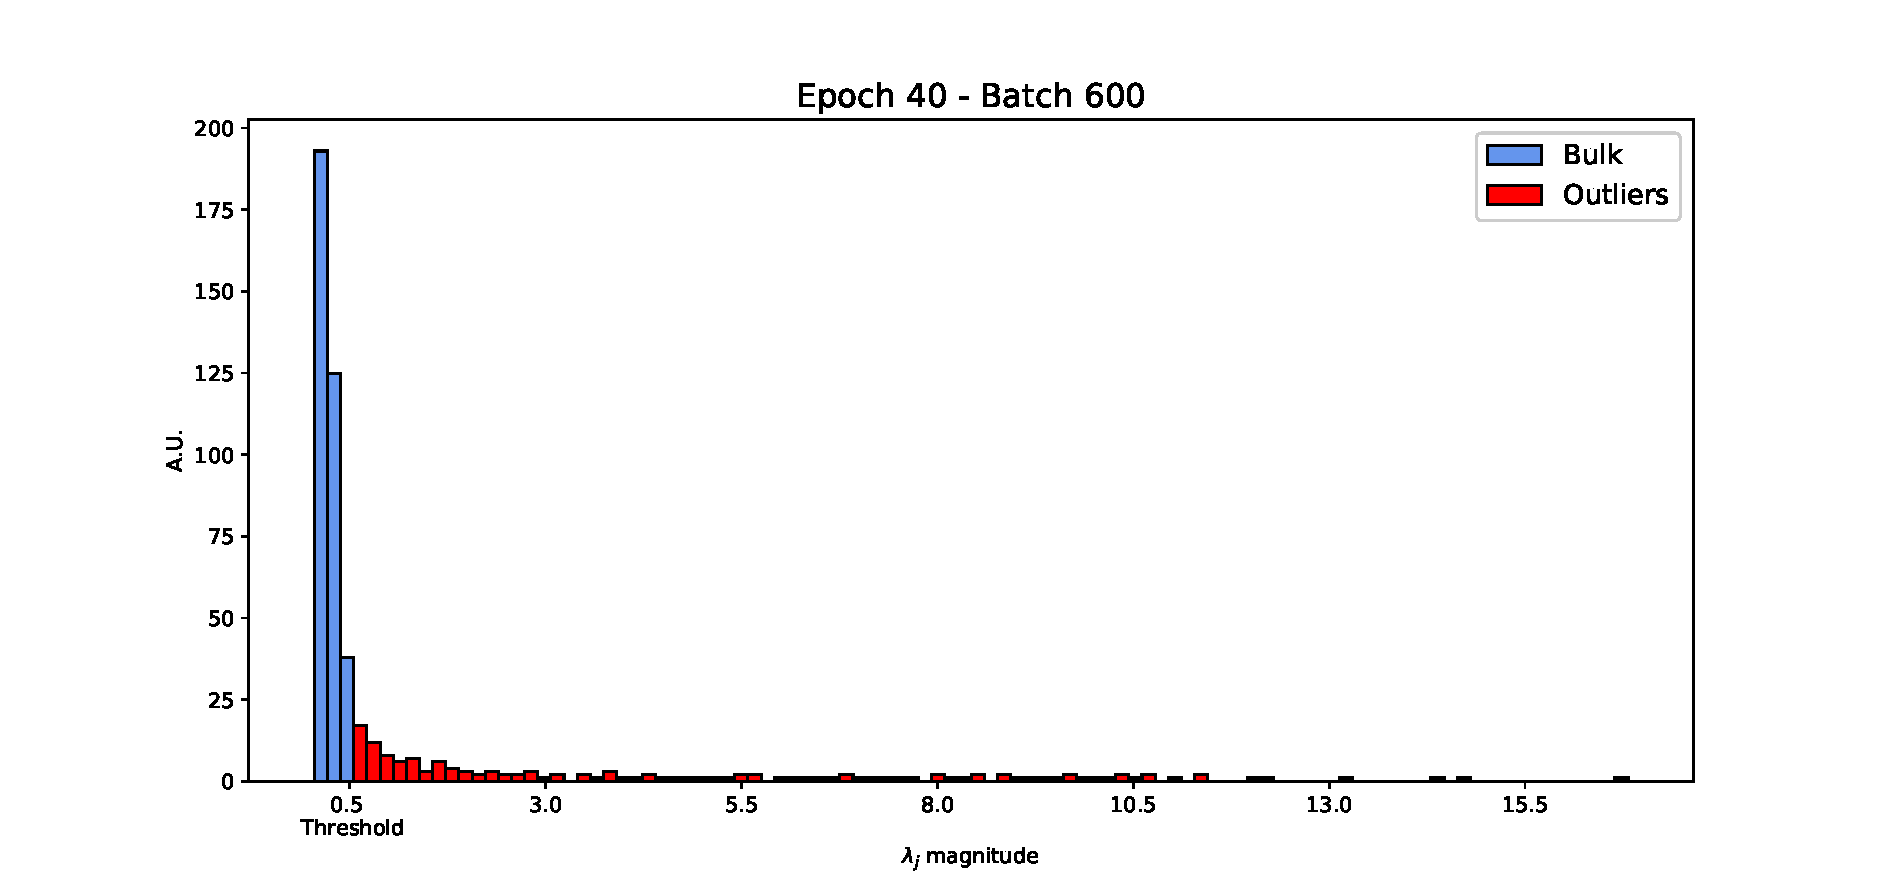
\includegraphics[width=\linewidth]{sv_distr_e40_b600.eps}
    \caption{}  
    \label{fig:sv4}
  \end{subfigure}
 \caption{\textbf{(a)} Singular values distribution of the initial random matrix compared to Marchenko-Pastur law. \textbf{(b)-(d)} With the training we can see some singular values strengthening and overcoming the threshold set by the Marchenko-Pastur law. \textbf{(e)} Distribution of the singular values after a long training: we can see many outliers spread above threshold and a spike of below-threshold singular values near zero}
\end{figure}

Starting with the training we see that many singular values increase in magnitude and overcome the threshold for a gaussian random matrix; these are \textit{outliers} leaving the bulk, shown in fig. \ref{fig:sv1}-\ref{fig:sv3}. During the first epochs of the training this process is very fast and many \(\sigma_j\) are easily extracted from the bulk, growing of many orders of magnitude. The bulk is instead shrinked to low values, meaning that the \(\sigma_j\) that do not overcome the threshold decrease in magnitude. Going on with the training this process slows down but it does not stop: outliers keep growing slowly and the bulk keeps shrinking to approach a spike around zero. It is important to note that a kind of hierarchy is maintained in the process: the first outliers are never overcome by the newly extracted \(\sigma_j\), and this is made clear by looking at the corresponding left singular vectors (see next section).
After a long training the singular values \(\sigma_j\) are separated into two categories: a concentrated set of almost-null singular values and a set of outliers spread above the threshold, as shown in fig. \ref{fig:sv4}.

The evolution of the \(\sigma_j\) distribution described above suggests that the training process is able to discern between the \textit{most important} singular vectors, that are brought above threshold first and heavily strengthen, and a bulk of \textit{less important} singular vectors, that end up above threshold but whose \( \sigma_j\) reach values order of magnitude smaller then those of the strongest singular vectors. Moreover, the below-threshold singular vectors are practically eliminated by cutting down the corresponding \(\sigma_j\).

These observations give a good indication about what are the dynamics of the learning process, but there are some matters that need to be addressed: (i) it is not clear what singular vectors actually represent, (ii) the meaning of \textit{more} and \textit{less} important singular vectors has to be specified, (iii) no clues about stopping criteria for the learning are given.

\subsection{Analysis of left singular vectors}

To understand the role of the left singular vectors of a RBM we must keep in mind the interpretation for the SVD decomposition of \textbf{W} given previously. We have seen how the matrix of the weights \textbf{\(\Sigma\)} is shaped during the learning, and we recall that \textbf{V} is interpreted as a rotation in the space of the hidden units. We then expect to recover the structure of the training data into the \textbf{U} matrix, and to show this we carefully analyze the left singular vectors during training by visualizing them in the pixel space.

Before focusing on the left singular vectors, we note that also the external visible field can be visualized in the pixel space. With the initialization rule \eqref{eq:bias_init} we are able to encode into the field the mean activation of the visible layer, which is clearly shown in fig. \ref{fig:vbias} in the pixel space. If we instead initialize the visible field with a null vector, the mean activation pattern is learnt very effectively as the strongest left singular vector. The striking resemblance between the mean activation pattern computed from the training data and the one learnt by the RBM is shown in fig. \ref{fig:m1tr}-\ref{fig:vbias} and it serves as a first example of what the left singular vectors represent. It seems then equivalent to either encode the mean activation pattern into the visible field since the beginning or letting the RBM learn such a pattern as a left singular vector. In practice the second case is not desirable as the RBM associates to the mean activation pattern a very strong singular value, many order of magnitudes higher then the strongest outliers. This results in a bias in the sampling from the trained machine, such that the samples whose activation pattern is nearest to the mean are sampled with a higher frequency (in the worst case those are the only configurations sampled at equilibrium).

\begin{figure}
  \centering
  \begin{subfigure}{.3\linewidth}
    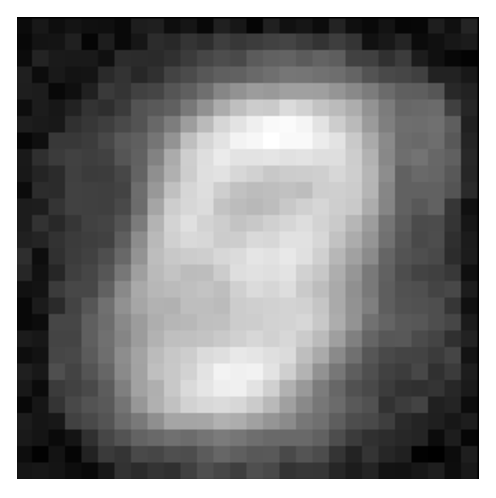
\includegraphics[width=\linewidth]{mode_1_training.eps}
    \caption{}
    \label{fig:m1tr}
  \end{subfigure}
  \begin{subfigure}{.3\linewidth}
    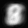
\includegraphics[width=\linewidth]{vbias.png}
    \caption{}
    \label{fig:vbias}
  \end{subfigure}
  \begin{subfigure}{.3\linewidth}
    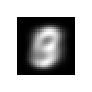
\includegraphics[width=\linewidth]{X_l_eigv_1.eps}
    \caption{}
    \label{fig:m1data}
  \end{subfigure}\par\medskip
  \begin{subfigure}{\linewidth}
    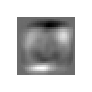
\includegraphics[width=.1\linewidth]{W_l_eigv_2.eps}
    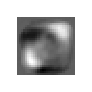
\includegraphics[width=.1\linewidth]{W_l_eigv_3.eps}
    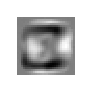
\includegraphics[width=.1\linewidth]{W_l_eigv_4.eps}
    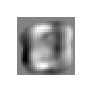
\includegraphics[width=.1\linewidth]{W_l_eigv_5.eps}
    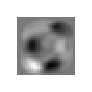
\includegraphics[width=.1\linewidth]{W_l_eigv_6.eps}
    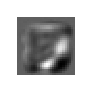
\includegraphics[width=.1\linewidth]{W_l_eigv_7.eps}
    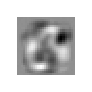
\includegraphics[width=.1\linewidth]{W_l_eigv_8.eps}
    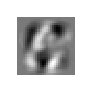
\includegraphics[width=.1\linewidth]{W_l_eigv_9.eps}
    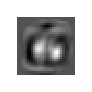
\includegraphics[width=.1\linewidth]{W_l_eigv_10.eps}
    \caption{}
    \label{fig:modes_tr}
  \end{subfigure}\par
  \begin{subfigure}{\linewidth}
    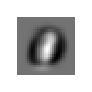
\includegraphics[width=.1\linewidth]{X_l_eigv_2.eps}
    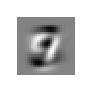
\includegraphics[width=.1\linewidth]{X_l_eigv_3.eps}
    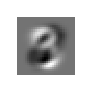
\includegraphics[width=.1\linewidth]{X_l_eigv_4.eps}
    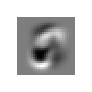
\includegraphics[width=.1\linewidth]{X_l_eigv_5.eps}
    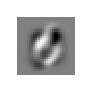
\includegraphics[width=.1\linewidth]{X_l_eigv_6.eps}
    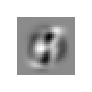
\includegraphics[width=.1\linewidth]{X_l_eigv_7.eps}
    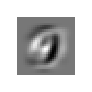
\includegraphics[width=.1\linewidth]{X_l_eigv_8.eps}
    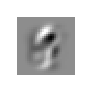
\includegraphics[width=.1\linewidth]{X_l_eigv_9.eps}
    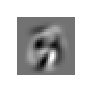
\includegraphics[width=.1\linewidth]{X_l_eigv_10.eps}
    \caption{}
    \label{fig:modes_data}
  \end{subfigure}
 \caption{\textbf{(a)} First mode learnt by the RBM with the external visible field initialized as a null vector. \textbf{(b)} External visible field initialized with rule \eqref{eq:bias_init}. \textbf{(c)} First principal components extracted from the training set. \textbf{(d)} The first 9 modes of a trained RBM when rule \eqref{eq:bias_init}  has been used. \textbf{(e)} Principal components extracted from the training set (starting from the second).}
\end{figure}

The first 10 left singular vectors of a trained RBM are shown in fig. \ref{fig:modes_tr}. They are all composed by a homogeneous background on the borders and a set of alternating dark and light traits in the center, highlighting the fact that each singular vector acts globally on the visible layer. Even if the pictures seen in fig. \ref{fig:modes_tr} are quite different one from another, an interesting trend is found: a higher number of alternating traits is present in the successive vectors. At this point it is useful to draw a comparison to the Fourier decomposition of an image and interpret the left singular values as the \textit{modes} composing the activation pattern. The first singular vectors, characterized by a small number of alternating traits, play the role of the \textit{low frequency} modes while the successive modes act as \textit{high frequency} modes. The analogy to Fourier modes is suggested by the fact that we are basically performing Principal Component Analysis (PCA) over the matrix \textbf{W} and the left singular vectors can thus be identified with the principal modes of variation.

Looking at the dynamics of the learning it is seen that the modes take shape one by one as the corresponding singular value \(\sigma_j\) is brought above threshold. The subsequent strengthening of the \(\sigma_j\) corresponds to refinements and rotations, with little effects on the characterization of the modes as high or low frequency modes. For what concerns the modes below threshold, they present a dark border and a random configuration in the center; in this case the only effect of the training is to discern what are the units which are never activated and no information about the actual structure of the data is found.

These observations suggest that the RBM is able to learn the modes that compose the activation patterns of the data, starting with the low frequency modes and proceeding with the high frequency ones. Moreover, with reference to the \(\sigma_j\) distribution (fig. \ref{fig:sv4}), we note that the low frequency modes are given a higher weigth.

Summarizing, the analysis of the left singular vectors gives many insights on the training procedure:

\begin{itemize}
\item a RBM is able to learn the modes that compose the activation patterns of the training data
\item the low frequency modes are learnt first and are given higher weigths
\item by continuing the training, new modes at increasing higher frequency are learnt while the already learnt modes are strengthen
\item the external visible field is equivalent to a left singular vector but we can avoid to learn it by using the appropriate initial conditions
\end{itemize}

Finally, the above observations suggest that the weights matrix of a trained RBM is composed by two classes of modes and we can express its components as

\begin{equation}
w_{i,j} = \sum_{\alpha \in bulk} \sigma_{\alpha} u_{i,\alpha} v_{j,\alpha} + \sum_{\alpha \in outliers} \sigma_{\alpha} u_{i,\alpha} v_{j,\alpha} 
\end{equation}

where \(u_{i,j}\) and \(v_{i,j}\) are the components of the \(\mathbf{U}\) and \(\mathbf{V}\) matrices of the SVD of \(\mathbf{W}\).

\section{Role of the modes}
By looking at the singular values distribution of \textbf{W} we have seen that there seem to be \textit{more} and \textit{less important} singular vectors. In the previous section we have then refined this observation by highlighting how the lowest-frequency modes are given the highest weights. We can then identify the more (less) important modes as the low (high) frequency ones. To gain some intuition about the meaning of this separation we can take our analogy further and think about the Fourier decomposition of a square wave; in such a case, the superposition of the low frequency harmonics is sufficient to build a good approximation of a square wave, while the role of the high frequency harmonics is that of sharpening the waveform at the discontinuity points. In the context of a trained RBM, we then expect that good approximations to the training data are obtained by exploiting only the low frequency modes, while the high frequency modes should represent minor corrections.

It is not clear, however, how we can discern between high and low frequency modes. Some hints to address this issue are given by looking at the value of the \(\sigma_j\) in decreasing order on a log-log plot (fig. x), in which an interesting picture emerges: the strongest \(\sigma_j\) are located far above threshold and are of comparable magnitude, followed by a tail of exponentially damped \(\sigma_j\). This picture is consistent across the training, the only difference being the damping cutoff that is increasing with the epochs. After a long training, however, the increase in the cutoff is very slow and this could serve as a signal to stop the learning, as such situation amounts to slowly strengthening singular values which are exponentially less important then the already learnt modes.

We are then driven to define the more important low frequency modes as the modes before cutoff, and the exponentially less important high frequency modes as those after cutoff. A consistency check is shown in fig. \ref{fig:hf_modes}, where just the 100 strongest modes are retained to construct the samples and the remaining modes are shown to encode boundary corrections. Choosing the first 100 modes is arbitrary; in fig. x we can see how the cutoff is well below 100, so with this choice we are sure that we included in the reconstruction of the samples all the strong modes before cutoff plus a small number of modes giving boundary corrections.

\begin{figure}
  \begin{subfigure}{\linewidth}
  	\centering
    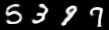
\includegraphics[width=.8\linewidth]{complete40ep.png}
    \caption{}
  \end{subfigure}\par
  \begin{subfigure}{\linewidth}
  	\centering
    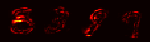
\includegraphics[width=.8\linewidth]{difference20ep.png}
    \caption{}  
  \end{subfigure}\par
  \begin{subfigure}{\linewidth}
  	\centering
    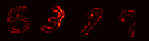
\includegraphics[width=.8\linewidth]{difference40ep.png}
    \caption{}
  \end{subfigure}
  \caption{\textbf{(a)} The image shows some samples obtained with the trained RBM (after a 40 epochs training) and then "filtered" by eliminating the 400 weakest modes (just the 100 strongest modes are retained). \textbf{(b)} The images are composed by eliminating the 100 strongest modes to see what the weakest modes actually encode (20 epochs training). \textbf{(c)} As in \textbf{(b)} but after a 40 epochs training.}
  \label{fig:hf_modes}
\end{figure}

 
\begin{thebibliography}{9}

\bibitem{go}
D. Silver et al., "Mastering the game of Go with deep neural networks and tree search",
\textit{Nature}, 529, p. 484–489, 2016.

\bibitem{foundations}
F. Cucker, S. Smale, "On the mathematical foundations of learning",
\textit{Bull. Amer. Math. Soc.}, 39, p. 1-49, 2002.

\bibitem{hist1}
W. Krauth, M. Mezard, "Machine Learning algorithms with optimal stability in neural networks",
\textit{Journal of Physics A: Mathematical and General}, 20, L745–L752, 1987.

\bibitem{hist2}
J. J. Hopfield, "Neural networks and physical systems with emergent collective computational abilities"\textit{Proceedings of the National Academy of Sciences, 79}, 8, p. 2554–2558, 1982.

\bibitem{tap_train}
M. Gabri\'e, E. W. Tramel, F. Krzakala,
Training Restricted Boltzmann Machines via the Thouless-Anderson-Palmer Free Energy,
\textit{Advances in Neural Information Processing Systems (NIPS)}, 28, pages 640--648, 2015.

\bibitem{tap}
E. W. Tramel, M. Gabri\'e, A. Manoel, F. Caltagirone, F. Krzakala, \textit{arXiv:1702.03260}

\bibitem{monasson}
J. Tubiana, R. Monasson, "Emergence of Compositional Representations in Restricted Boltzmann Machines",
\textit{Phys. Rev. Lett. 118, 138301}, 2017.

\bibitem{Hinton_CD}
G. E. Hinton, “Training products of experts by minimizing Contrastive divergence,”
\textit{Neural computation}
, vol. 14, pp. 1771-1800, 2002.

\bibitem{PCD}
T. Tieleman, “Training restricted Boltzmann machines using approximations to the likelihood gradient,”
\textit{ICML}, Vol. 307, p. 7, 2008.

\bibitem{Hinton_guide}
G. E. Hinton, "A Practical Guide to Training Restricted Boltzmann Machines", \textit{Proceedings of Neural Networks: Tricks of the Trade (2nd ed.)}, pages 599-619, 2012. 

\bibitem{PCA}
I.T. Jolliffe, "Principal Component Analysis",
\textit{Springer-Verlag New York}, 2002.

\bibitem{SK}
D. Sherrington, S. Kirkpatrick,
"Solvable Model of a Spin-Glass",
\textit{Phys. Rev. Lett.}, Vol. 35, 1975.

\bibitem{ht_exp}
A. Georges, J. S. Yedidia,
"How to expand around mean-field theory using high-temperature expansions",
\textit{Journal of Physics A: Mathematical and General}, Volume 24, Number 9, 1991

\bibitem{TAP}
D. J. Thouless , P. W. Anderson, R. G. Palmer,
"Solution of 'Solvable model of a spin glass'",
\textit{Philosophical Magazine}, Vol. 35:3, p. 593-601, 1977

\bibitem{conv}
E. Bolthausen, "An Iterative Construction of Solutions of the TAP Equations for the Sherrington–Kirkpatrick Model", \textit{Commun. Math. Phys.}, Vol. 325, pages 333-366, 2014.

\bibitem{mnist}
http://yann.lecun.com/exdb/mnist/

\bibitem{gibbs}
G. Casella and E. I. George, "Explaining the Gibbs Sampler",
\textit{The American Statistician},
Vol. 46, No. 3, pp. 167-174, 1992.

\bibitem{leroy}
C. Leroy made an investigation on TAP fixed points and free energy landscape while at Laboratoire de Recherche en Informatique, working in my same team.

\bibitem{Nishimori}
H. Nishimori, "Statistical Physics of Spin Glasses and Information Processing: An Introduction",
\textit{Oxford University Press}, 2001

\bibitem{MP_law}
Marchenko, V.A. and Pastur, L.A., "Distribution of Eigenvalues for Some Sets of Random Matrices", \textit{Sbornik: Mathematics}, Vol. 1, pages 457-483, 1967.

\bibitem{ganguli}
A. M. Saxe, J. L. McClelland, S. Ganguli, "Exact solutions to the nonlinear dynamics of learning in deep linear neural networks",
\textit{arXiv:1312.6120}, 2014.

\end{thebibliography}


\end{document}
